\chapter{Supplementary Information Chapter 4}\label{apx:ch4}

\begin{figure*}[htb]
  \centering
    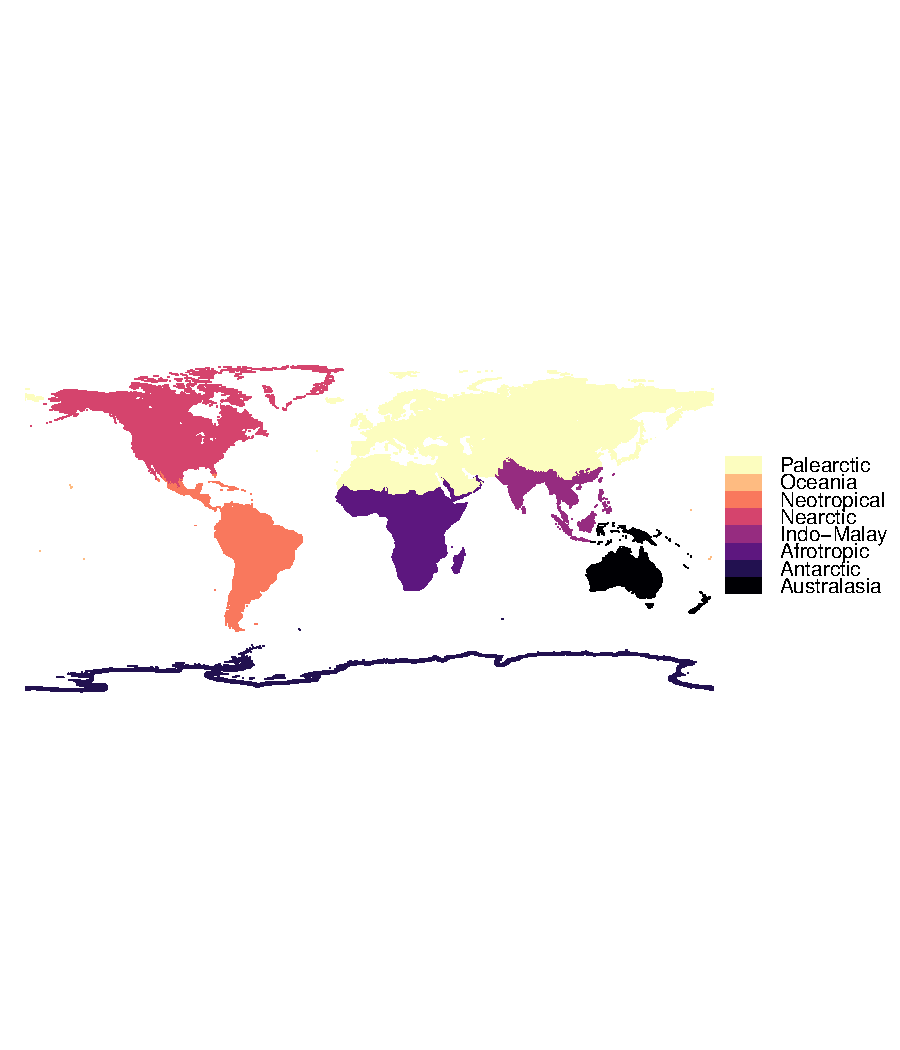
\includegraphics{chapters/figures/chapter4/supfig_ecorealms.pdf} 
    \caption{Biogeographic realms used for the aggregation of biodiversity predictions.}
    \label{ch4:supfig_ecorealms}
\end{figure*}

\begin{table}[htb]
\centering
\caption{Relative contributions of commodity sectors to the total area harvested in 2019. These values inform the weight of predicted land endowment changes when estimating total changes to crop land area. c\_b: sugar cane, sugar beet; gro: Cereal grains nec; ocr: Crops nec; osd: oil seeds; pdr: paddy rice; pfb: plant-based fibres; v\_f: vegetables, fruit, nuts; wht: wheat.}
\label{apx:ch4:tab_faoharvested}
\begin{tabularx}{0.7\textwidth}{lllllllll}
\toprule
region & c\_b & gro & ocr & osd & pdr & pfb & v\_f & wht \\
\bottomrule
aus & 2.01 & 28.34 & 7.7 & 10.18 & 0.04 & 1.41 & 2.16 & 48.17 \\
xoc & 2.63 & 0.41 & 2.08 & 14.97 & 0.26 & 8.43 & 71.21 & 0.01 \\
chn & 0.92 & 23.82 & 2.3 & 11.93 & 16.26 & 4.49 & 27.35 & 12.94 \\
jpn & 0.74 & 2.14 & 1.62 & 5.25 & 53.33 & 3.37 & 26.24 & 7.32 \\
kor & 2.16 & 4.19 & 3.41 & 4.34 & 49.89 & 0.17 & 35.56 & 0.27 \\
xea & NA & 24.59 & 15.37 & 5.4 & 15.44 & 0.65 & 27.18 & 11.37 \\
mys & 2.14 & 0.1 & 0.29 & 84.96 & 9.23 & 0.22 & 3.06 & NA \\
phl & 2.63 & 16.75 & 0.71 & 2.11 & 30.95 & 0.21 & 46.64 & NA \\
tha & 8.94 & 5.61 & 1.39 & 20.72 & 47.3 & 0.15 & 15.88 & 0.01 \\
vnm & 1.68 & 7.14 & 4.21 & 6.83 & 53.73 & 0.84 & 25.57 & NA \\
idn & 0.94 & 13.54 & 2.28 & 41.15 & 22.55 & 3.62 & 15.92 & NA \\
xse & 1.04 & 5.49 & 23.34 & 9.62 & 45.79 & 1.14 & 13.33 & 0.25 \\
ind & 2.6 & 11.07 & 15.11 & 11.92 & 21.88 & 8.38 & 14.39 & 14.65 \\
xsa & 2.19 & 10.88 & 4.52 & 3.1 & 28.1 & 4.91 & 14.19 & 32.11 \\
can & 0.02 & 18.41 & 11.64 & 36.72 & NA & 0.04 & 1.3 & 31.86 \\
usa & 0.39 & 38.25 & 1.43 & 34.09 & 1.05 & 5.44 & 3.55 & 15.81 \\
mex & 5.27 & 55.19 & 9.49 & 2.26 & 0.25 & 1.74 & 21.96 & 3.84 \\
bra & 12.52 & 23.8 & 4.56 & 44.92 & 2.1 & 2.72 & 6.8 & 2.58 \\
xsm & 3.53 & 22.5 & 4.33 & 37.64 & 4.1 & 2.36 & 15.42 & 10.12 \\
fra & 0.08 & 29.16 & 2.42 & 15.01 & 0.11 & 3.29 & 11.27 & 38.66 \\
deu & 0.06 & 38.49 & 2 & 10.8 & 0 & 4.84 & 6.84 & 36.96 \\
gbr & NA & 31.33 & 4.02 & 12.43 & NA & 2.44 & 8.8 & 40.98 \\
rus & 0.11 & 23.6 & 3.42 & 21.97 & 0.3 & 1.8 & 5.14 & 43.66 \\
e25 & 0.39 & 33.35 & 2.44 & 18.56 & 0.76 & 1.37 & 17.55 & 25.58 \\
xsu & 0.07 & 24.71 & 2.22 & 21.16 & 0.63 & 4.02 & 9.07 & 38.12 \\
xer & 0.09 & 35.5 & 1.67 & 24.38 & 0.28 & 0.52 & 11.76 & 25.78 \\
xws & 0.21 & 26.99 & 5.98 & 9.64 & 0.9 & 3.39 & 18.03 & 34.86 \\
xnf & 0.54 & 35.43 & 14.58 & 16.66 & 1.95 & 2.76 & 11.59 & 16.48 \\
ssa & 0.9 & 32.38 & 19.34 & 10.46 & 6.64 & 6.45 & 22.71 & 1.12 \\
xtw & 0.92 & 11.54 & 1.89 & 2.39 & 28.64 & 1.25 & 48.34 & 5.04 \\
\bottomrule
\end{tabularx}
\end{table}

\begin{table}[htb]
\centering
\caption{Mapping of Global Land Systems (GLS) classes with land use classes and intensity classes. Table adopted from \citet{newbold_global_2015}.}
\label{apx:ch4:tab_glsmapping}
\begin{tabularx}{1\textwidth}{Ylllll}
\toprule
Global Land Systems classification & Primary & Secondary & Cropland & Pasture & Urban \\
\bottomrule
Cropland, extensive with few livestock & NA & NA & minimal & light & NA \\
Cropland, extensive with bovines, goats \& sheep & NA & NA & minimal & intense & NA \\
Cropland, extensive with pigs \& poultry & NA & NA & minimal & intense & NA \\
Cropland, medium intensive with few livestock & NA & NA & light & light & NA \\
Cropland, medium intensive with bovines, goats \& sheep & NA & NA & light & intense & NA \\
Cropland, medium intensive with pigs \& poultry & NA & NA & light & intense & NA \\
Cropland, intensive with few livestock & NA & NA & intense & light & NA \\
Cropland, intensive with bovines, goats \& sheep & NA & NA & intense & intense & NA \\
Cropland, intensive with pigs \& poultry & NA & NA & intense & intense & NA \\
Mosaic cropland and grassland with bovines, goats and sheep & NA & NA & intense & intense & NA \\
Mosaic cropland and grassland with pigs \& poultry & NA & NA & intense & intense & NA \\
Mosaic cropland (extensive) and grassland with few livestock & NA & NA & minimal & light & NA \\
Mosaic cropland (medium intensive) and grassland with few livestock & NA & NA & light & light & NA \\
Mosaic cropland (intensive) and grassland with few livestock & NA & NA & intense & light & NA \\
Mosaic cropland and forest with pigs \& poultry & NA & NA & intense & intense & NA \\
Mosaic cropland (extensive) and forest with few livestock & NA & NA & minimal & light & NA \\
Mosaic cropland (medium intensive) and forest with few livestock & NA & NA & light & light & NA \\
Mosaic cropland (intensive) and forest with few livestock & NA & NA & intense & light & NA \\
Dense forest & minimal & minimal & NA & NA & NA \\
Open forest with few livestock & light & light & NA & light & NA \\
Open forest with pigs \& poultry & intense & intense & NA & intense & NA \\
Mosaic grassland and forest & minimal & minimal & NA & NA & NA \\
Mosaic grassland and bare & minimal & minimal & NA & NA & NA \\
Natural grassland & minimal & minimal & NA & NA & NA \\
Grassland with few livestock & NA & NA & NA & light & NA \\
Grassland with bovines, goats and sheep & NA & NA & NA & intense & NA \\
Bare & NA & NA & NA & NA & NA \\
Bare with few livestock & NA & NA & NA & light & NA \\
Peri-urban and villages & NA & NA & NA & NA & minimal \\
Urban & NA & NA & NA & NA & intense \\
\bottomrule
\end{tabularx}
\end{table}

\begin{landscape}
\begin{table}[htb]
\captionsetup{width=1.5\textwidth}
\centering
\caption{Description of land use types and intensities. Table adopted from \citet{newbold_global_2015} and originally based on \citet{hudson_predicts_2014}. In this study, we combined different secondary vegetation types into one class, because the applied land use model was unable to explicitely model succession between secondary vegetation stages.}
\label{apx:ch4:tab_intensity}
\begin{tabularx}{1.5\textwidth}{YlYYY}
\toprule
Level 1 Land Use &
  Predominant Land use &
  Minimal use &
  Light use &
  Intense use \\
  \bottomrule
\makecell[lt]{No evidence of prior destruction \\ of the vegetation \\ \\ Recovering after destruction \\ of the vegetation} &
  \makecell[lt]{Primary Vegetation \\ \\ \\ Secondary Vegetation} & Any disturbances identified are very minor (e.g., a trail or path) or very limited in the scope of their effect (e.g., hunting of a particular species of limited ecological importance). & 
  One or more disturbances of moderate intensity (e.g., selective logging) or breadth of impact (e.g., bushmeat extraction), which are not severe enough to markedly change the nature of the ecosystem. Primary sites in suburban settings are at least Light use. &
  One or more disturbances that are severe enough to markedly change the nature of the ecosystem; this includes clear- felling of part of the site too recently for much recovery to have occurred. Primary sites in fully urban settings should be classed as Intense use. \\
Human use (agricultural) &
  Plantation forest &
  Extensively managed or mixed timber, fruit/coffee, oil-palm or rubber plantations in which native understorey and/or other native tree species are tolerated, which are not treated with pesticide or fertiliser, and which have not been recently (\textless 20 years) clear- felled. &
  Monoculture fruit/coffee/rubber plantations with limited pesticide input, or mixed species plantations with significant inputs. Monoculture timber plantations of mixed age with no recent (\textless 20 years) clear-felling. Monoculture oil-palm plantations with no recent (\textless 20 years) clear-felling. &
  Monoculture fruit/coffee/rubber plantations with significant pesticide input. Monoculture timber plantations with similarly aged trees or timber/oil-palm plantations with extensive recent (\textless 20 years) clear-felling. \\
 &
  Cropland &
  Low-intensity farms, typically with small fields, mixed crops, crop rotation, little or no inorganic fertiliser use, little or no pesticide use, little or no ploughing, little or no irrigation, little or no mechanisation. &
  Medium intensity farming, typically showing some but not many of the following: large fields, annual ploughing, inorganic fertiliser application, pesticide application, irrigation, no crop rotation, mechanisation, monoculture crop. Organic farms in developed countries often fall within this category, as may high- intensity farming in developing countries. &
  High-intensity monoculture farming, typically showing many of the following features: large fields, annual ploughing, inorganic fertiliser application, pesticide application, irrigation, mechanisation, no crop rotation. \\
 &
  Pasture &
  Pasture with minimal input of fertiliser and pesticide, and with low stock density (not high enough to cause significant disturbance or to stop regeneration of vegetation). &
  Pasture either with significant input of fertiliser or pesticide, or with high stock density (high enough to cause significant disturbance or to stop regeneration of vegetation). &
  Pasture with significant input of fertiliser or pesticide, and with high stock density (high enough to cause significant disturbance or to stop regeneration of vegetation). \\
Human use (urban) &
  Urban &
  Extensive managed green spaces; villages. &
  Suburban (e.g. gardens), or small managed or unmanaged green spaces in cities. &
  Fully urban with no significant green spaces.\\
  \bottomrule
\end{tabularx}
\end{table}
\end{landscape}


% Please add the following required packages to your document preamble:
% \usepackage{lscape}
\begin{table}[htb]
\centering
\caption{Fraction of cells ($\%$) chosen in each time step for the new establishment of land use types (chosen cells were completely devoid of that land use in the preceding time step). Values derived from observed time steps 1990-2005 \citep{hurtt_harmonization_2011}.}
\label{apx:ch4:tab_newest}
\begin{tabularx}{0.55\textwidth}{lllllY}
\toprule
region & cropland & pasture & primary & secondary & urban \\
\bottomrule
aus    & 0.000    & 0.000   & 0.000   & 0.000     & 1.193 \\
xoc    & 0.291    & 0.000   & 0.011   & 1.058     & 0.422 \\
chn    & 0.119    & 0.000   & 0.100   & 2.672     & 0.408 \\
jpn    & 0.000    & 0.000   & 0.000   & 0.000     & 0.000 \\
kor    & 0.518    & 0.000   & 0.003   & 1.044     & 0.139 \\
xea    & 0.411    & 0.000   & 0.005   & 0.125     & 0.520 \\
mys    & 0.000    & 0.000   & 0.000   & 0.321     & 0.064 \\
phl    & 0.499    & 0.000   & 0.056   & 0.438     & 0.137 \\
tha    & 0.243    & 0.000   & 0.004   & 0.413     & 0.226 \\
vnm    & 0.051    & 0.000   & 0.000   & 0.000     & 0.076 \\
idn    & 0.000    & 0.000   & 0.000   & 0.466     & 0.055 \\
xse    & 0.041    & 0.000   & 0.000   & 0.000     & 1.282 \\
ind    & 0.442    & 0.000   & 0.008   & 0.046     & 0.564 \\
xsa    & 1.639    & 0.000   & 0.000   & 0.341     & 0.199 \\
can    & 0.000    & 0.000   & 0.000   & 0.018     & 0.388 \\
usa    & 0.164    & 0.000   & 0.000   & 0.078     & 0.418 \\
mex    & 1.481    & 0.000   & 0.238   & 0.733     & 0.007 \\
bra    & 0.000    & 0.000   & 0.000   & 0.000     & 0.204 \\
xsm    & 0.000    & 0.000   & 0.000   & 0.196     & 0.980 \\
fra    & 0.124    & 0.000   & 0.000   & 0.000     & 0.321 \\
deu    & 0.317    & 0.000   & 0.005   & 0.034     & 0.790 \\
gbr    & 0.743    & 0.000   & 0.012   & 0.138     & 0.321 \\
rus    & 0.232    & 0.000   & 0.110   & 0.844     & 0.245 \\
e25    & 0.000    & 0.000   & 0.000   & 0.000     & 0.819 \\
xsu    & 3.041    & 0.000   & 0.026   & 0.137     & 0.077 \\
xer    & 0.417    & 0.000   & 0.417   & 0.000     & 0.052 \\
xws    & 0.000    & 0.000   & 0.000   & 3.717     & 0.040 \\
xnf    & 0.925    & 0.000   & 0.009   & 2.112     & 0.780 \\
ssa    & 0.057    & 0.000   & 0.000   & 0.000     & 0.115 \\
xtw    & 0.990    & 0.000   & 0.028   & 0.182     & 0.149 \\
\bottomrule
\end{tabularx}
\end{table}

    
\begin{figure*}[htb]
  \centering
    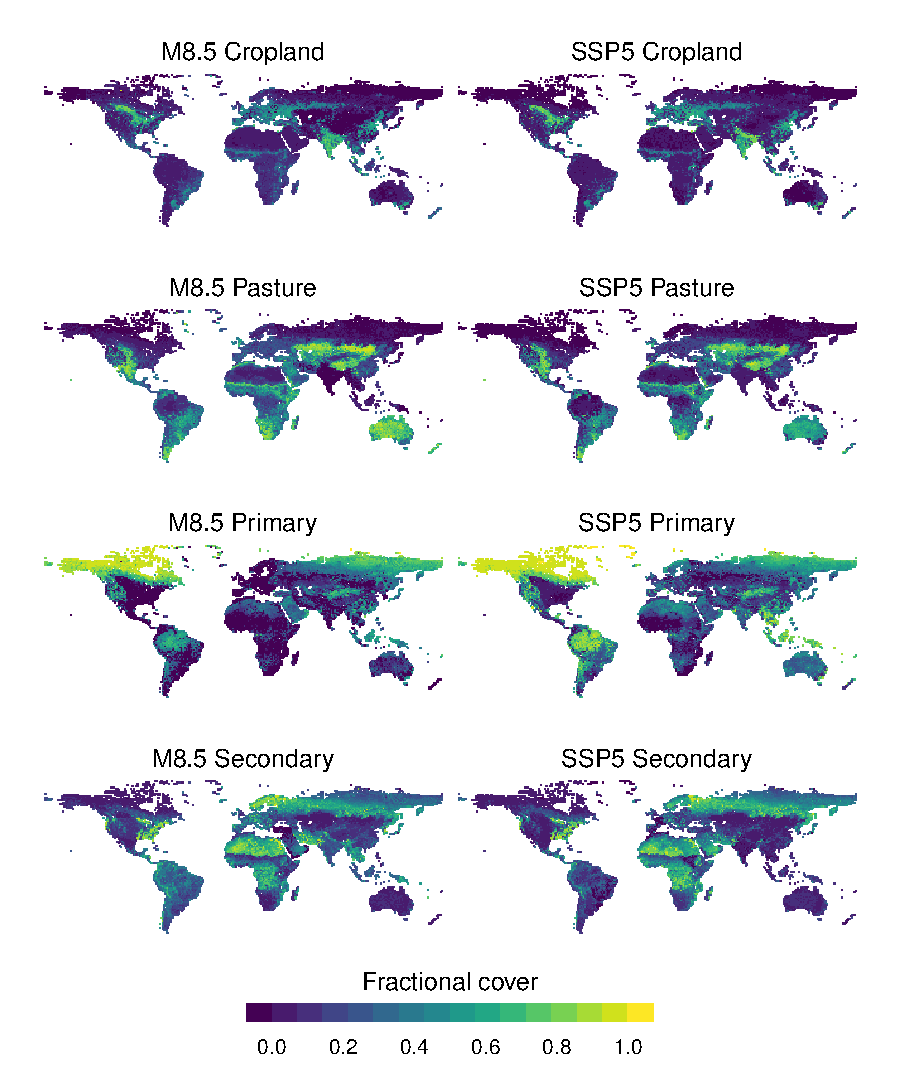
\includegraphics{chapters/figures/chapter4/fig_landusemaps.pdf}
    \caption{land-use.}
    \label{ch4:fig_landusemaps}
\end{figure*}
    
